\documentclass[./Thesis.tex]{subfiles}
\begin{document}

\chapter{Termination}
\label{chap:termination}

\epigraph{
  What can be asserted without evidence can also be dismissed without evidence.
}{Christopher Hitchens \cite{hitchens-quote}}

\begin{code}[hide]
  module Termination where
  open import Relation.Nullary using (¬_)
  open import Relation.Nullary.Decidable using (False)
  open import Relation.Nullary.Negation using (contradiction)
  open import Data.Empty using (⊥)
  open import AKS.Nat using (ℕ; zero; suc; _∸_; _*_; _<_; _≤_; lte; _≟_)
  open import AKS.Nat using (+-comm; suc-injective-≡; n≮0; 0≤n; n<1+n; ≤-refl) renaming (n≤m⇒n<m⊎n≡m to n≤m⇒n<m∨n≡m)
  open import Data.Sum using () renaming (inj₁ to or₁; inj₂ to or₂)
  open import AKS.Binary using (𝔹⁺)
  open 𝔹⁺
  open import AKS.Nat.Divisibility using (_div_; Euclidean; Euclidean✓)
  open Euclidean using () renaming (q to quotient)
  open import Relation.Binary.PropositionalEquality
    using (_≡_; _≢_; module ≡-Reasoning)
    renaming (refl to ≡-refl; sym to ≡-sym; cong to ≡-cong; cong₂ to ≡-cong₂)
  open ≡-Reasoning
  open import Data.Unit using (tt)
  open import Polynomial.Simple.AlmostCommutativeRing.Instances using (module Nat)
  open import Polynomial.Simple.Reflection using (solve)
  open Nat.Reflection using (∀⟨_⟩)
  open import Data.List using ([]; _∷_; List)
  open import Function using (_$_)
  open import AKS.Unsafe using (BOTTOM)
\end{code} % $
\section{A Correctness Interlude}
\label{sec:a-correctness-interlude}
The previous chapter omitted a critical flaw in its analysis. The code below is
rejected by the \Agda{} compiler. The compiler's \textit{termination checker} \cite{agda}
fails as \Agda{} can not infer that the result of non-zero integer division by
two always returns an integer strictly smaller than the input. The termination
checker ensures than every function is total. In other words,
the termination checker disallows infinite loops. This termination proof
is obvious but termination proofs can quickly become complex. In general checking
termination, commonly called the halting problem, is undecidable. 
\begin{code}[hide]
  module Bad₁ where
    {-# TERMINATING #-}
\end{code}
\begin{code}
    ⟦_⇑⟧⁺ : ∀ (n : ℕ) {≢0 : False (n ≟ 0)} → 𝔹⁺
    ⟦ suc n ⇑⟧⁺ with suc n div 2
    ... | Euclidean✓ (suc q) 0 _ _ = ⟦ suc q ⇑⟧⁺ 0ᵇ
    ... | Euclidean✓ zero    1 _ _ = 𝕓1ᵇ
    ... | Euclidean✓ (suc q) 1 _ _ = ⟦ suc q ⇑⟧⁺ 1ᵇ
\end{code}
This checker is a keystone of the correctness of the logic of \Agda{}. Consider
the following function with a similar call graph. Instead of the input
decreasing to some base case it doubles with every recursive call. This function can
be used to prove falsehood, thus a logic with unconstrained recursion is
inconsistent.
\begin{code}[hide]
  module Bad₂ where
    {-# TERMINATING #-}
\end{code}
\begin{code}
    increasing : ℕ → ⊥
    increasing n with 2 * n
    ... | q = increasing q

    false : ⊥
    false = increasing 0
\end{code}
In fact the example above can be simplified in the following code. In English
this code expresses the famous fallacy of circular reasoning ``false is true
because false is true''.
\begin{code}[hide]
  module Bad₃ where
    {-# TERMINATING #-}
\end{code}
\begin{code}
    false : ⊥
    false = false
\end{code}
Thankfully none of these false expressions are accepted by the \Agda{} compiler.
This begs the question how does \Agda{} determine which recursive functions to
accept? Unfortunately the \Agda{} compiler can not solve the halting problem so
it must be restrictive. The compiler only accepts recursive
calls that are \textit{structurally decreasing}, a small
subset of the set of recursive functions. A recursive call is structurally
decreasing if the call occurs on a strict sub expression \cite{agda}. The
expression $\AgdaInductiveConstructor{suc} \, n$ is a strict sub-expression of
$\AgdaInductiveConstructor{suc} \,
  (\AgdaInductiveConstructor{suc} \,
    (\AgdaInductiveConstructor{suc} \, n))
$
but $\AgdaInductiveConstructor{suc} \, n$ is not a strict sub-expression of
$\AgdaInductiveConstructor{suc} \, n$.
Addition, our first example of recursion, is acceptable as
$n <_{sub} \AgdaInductiveConstructor{suc} \, n$.
\begin{code}[hide]
  module Add where
\end{code}
\begin{code}
    _+_ : ℕ → ℕ → ℕ
    zero + m = m
    (suc n) + m = suc (n + m)
\end{code}
\begin{code}[hide]
  open import AKS.Nat using (_+_)
\end{code}
The following inductive definition of the Fibonacci function
has structurally decreasing calls as
$\AgdaInductiveConstructor{suc} \, n <_{sub} \AgdaInductiveConstructor{suc} \, (\AgdaInductiveConstructor{suc} \, n)$
and
$n <_{sub} \AgdaInductiveConstructor{suc} \, (\AgdaInductiveConstructor{suc} \, n)$.
\begin{code}
  fib : ℕ → ℕ
  fib zero = 0
  fib (suc zero) = 1
  fib (suc (suc n)) = fib (suc n) + fib n
\end{code}
So far all the recursive functions described have been
\textit{primitive recursive} \cite{soare}. This is a large class but the set of
structurally decreasing functions is larger than the set of primitive
recursive functions. The Ackerrmann function is the canonical example of
function which is not primitive recursive.
\begin{code}
  ack : ℕ → ℕ → ℕ
  ack zero m = suc m
  ack (suc n) zero = ack n (suc zero)
  ack (suc n) (suc m) = ack n (ack (suc n) m)
\end{code}
\Agda{} accepts this definition as the recursive
calls are decreasing lexicographically.
The recursive call in the second case decreases in the first argument so
the second argument increasing is acceptable
$
(n, \, \AgdaInductiveConstructor{suc} \, \AgdaInductiveConstructor{zero})
<_{sub}
(\AgdaInductiveConstructor{suc} \, n, \, \AgdaInductiveConstructor{zero})
$.
For a similar reason the outer call in the third case is acceptable
$
(n, \, \AgdaFunction{ack} \, (\AgdaInductiveConstructor{suc} \, n) \, m)
<_{sub}
(\AgdaInductiveConstructor{suc} \, n, \, \AgdaInductiveConstructor{suc} \, m)
$.
The inner call is acceptable as the second argument decreases while the first
stays constant, this is lexicographic order
$
(\AgdaInductiveConstructor{suc} \, n, \, m)
<_{sub}
(\AgdaInductiveConstructor{suc} \, n, \, \AgdaInductiveConstructor{suc} \, m)
$. \\
\section{Well-Founded Relations}
\label{sec:well-founded-relations}
An astute reader may have noticed a pattern. \Agda{} accepts your recursive
definition if it can infer a structural \textit{well-founded relation}
\cite{soare}. A well-founded relation is a binary relation $\prec$ that has no
infinitely descending chains $\dots \prec x_k \prec \dots \prec x_1 \prec x_0$.
For instance the strict ordering over the naturals is well-founded
as every chain will eventually reach the zero natural.
\begin{align}
  \label{eqn:wellfounded-natural}
  0 < 1 < 2 < 3 < 4 < 5
\end{align}
The non strict ordering is not well-founded as an infinite chain of the
reflexivity axiom can be constructed.
\begin{align}
  \label{eqn:non-wellfounded-natural}
  \dots \leq 0 \leq \dots \leq 0 \leq 0
\end{align}
Unfortunately these relation chains do not capture the full structure of well-founded
relations. A well-founded relation often has multiple elements that could be
appended to the chain. This idea is illustrated in the well-founded tree
rooted at 3 found in figure \ref{fig:wellfounded-tree}.
\begin{figure}[h]
  \centering
  \begin{tikzpicture}
    \Tree
    [.3
      {$0 < 3$}
      [.{$1 < 3$}
        {$0 < 1$}
      ]
      [.{$2 < 3$}
        {$0 < 2$}
        [.{$1 < 2$}
          {$0 < 1$}
        ]
      ]
    ]
  \end{tikzpicture}
  \caption{A well-founded tree }
  \label{fig:wellfounded-tree}
\end{figure}
These trees encapsulate the full structure of a well-ordering relation.
Therefore if we could express this tree as an \Agda{} datatype we could supply
our own well-ordering relation even when \Agda{} can not infer it. The final
datatype that represents well-founded trees is somewhat puzzling at first
glance. So to introduce it we start with a sensible datatype and make small
changes to the definition until we have reached the correct representation.
These trees are general trees, trees that can have an arbitrary number
of children. They are often called rose trees in functional programming
literature. They make for a good starting datatype.
\begin{code}[hide]
  module Tree₁ where
\end{code}
\begin{code}
    data RoseTree : Set where
      Node : List RoseTree → RoseTree
\end{code}
We then apply a \textit{continuation passing style} \cite{harper} transformation to the
recursive call. Instead of having a list of children we have a continuation that
can be invoked with the index of the requested child.
\begin{code}[hide]
  module Tree₂ where
\end{code}
\begin{code}
    data RoseTree : Set where
      Node : (ℕ → RoseTree) → RoseTree
\end{code}
Unfortunately this makes our definition unusable as now every rose tree must have
infinite size. From a game theotertic perspective, a consumer may request
the first child of every node repetitively.
\begin{code}
    rosetree-uninhabited : RoseTree → ⊥
    rosetree-uninhabited (Node children) = rosetree-uninhabited (children 0)
\end{code}
Any well founded tree is necessarily finite as each node always has a finite
number of children ``less'' than itself. We can solve this by adding an upper
bound and ensuring that any index is less than the bound.
\begin{code}[hide]
  module Tree₃ where
\end{code}
\begin{code}
    data RoseTree (bound : ℕ) : Set where
      Node : (∀ {lower : ℕ} → lower < bound → RoseTree lower)
           → RoseTree bound
\end{code}
Note that the definition above does not make use of any properties specific to
natural numbers. The definition simply requires a binary relation.
By parameterizing the datatype by the relation we
arrive at our finial definition. This is often called the accessibility
predicate so we update the names accordingly.
\begin{code}
  data Acc {A : Set} (_≺_ : A → A → Set) (bound : A) : Set where
    acc : (∀ {lower : A} → lower ≺ bound → Acc _≺_ lower)
        → Acc _≺_ bound
\end{code}
Continuing with the game theoretic analysis proving a relation is well-founded
for a specific bound is a simple game. A game where the prover
continually asks for a lower bound and wins when it is impossible for the
other player to supply a lower bound. This game plays out below for a bound of $3$.
\begin{code}
  3-well-founded : Acc _<_ 3
  3-well-founded = acc λ l₁<3 → acc λ l₂<l₁ → acc λ l₃<l₂ → acc λ l₄<l₃ →
    contradiction l₄<l₃ (end l₁<3 l₂<l₁ l₃<l₂)
\end{code}
\begin{code}[hide]
    where
\end{code}
\begin{code}
    end : ∀ {l₁ l₂ l₃ l₄} → l₁ < 3 → l₂ < l₁ → l₃ < l₂ → ¬ (l₄ < l₃)
    end {2} {1} {0} {l₄} l₁<3 l₂<l₁ l₃<l₂ l₄<l₃ = contradiction l₄<l₃ n≮0 
\end{code}
\section{Win Every Game}
\label{sec:win-every-game}
Now we turn to proving that any natural forms a rooted well-founded tree under the
strict ordering relation. Usually proving a property holds for any $n$ is harder
then proving that property holds for specific $n$. This concept applies to
proving that every natural is well-founded. Specifically our choice of
less than relation is poorly suited for this task. We will define an inductive
ordering relation and show that our original definition of ordering is a
subrelation of the inductive-definition. Then if the inductive definition is
well-founded the subrelation will be as well. This last idea is shown below.
\begin{code}[hide]
  module Sub₁ where
\end{code}
\begin{code}
    subrelation
        : ∀ {A : Set} {_≺₁_ _≺₂_ : A → A → Set} {n}
        → (∀ {a b} → a ≺₂ b → a ≺₁ b)
        → Acc _≺₁_ n
        → Acc _≺₂_ n
    subrelation ≺₂⇒≺₁ (acc down) =
      acc λ x≺₂n → subrelation ≺₂⇒≺₁ (down (≺₂⇒≺₁ x≺₂n))
\end{code}
Next we turn to the inductive ordering relation. The key idea behind this
definition is that each $\AgdaInductiveConstructor{≤-step}$ constructor adds one
to the right bound. The base case is the reflexivity axiom so the number of
$\AgdaInductiveConstructor{≤-step}$ constructors is the distance between the
left and right bound. The old definition internalizes this concept into the
definition as the $k$ in
$a \, \AgdaDatatype{≤} \, b = a \, \AgdaFunction{+} \, k \, \AgdaDatatype{≡} \, b$.
\begin{code}
    data _≤ⁱ_ (n : ℕ) (m : ℕ) : Set where
      ≤-same : n ≡ m → n ≤ⁱ m
      ≤-step : ∀ {o} → suc o ≡ m → n ≤ⁱ o → n ≤ⁱ m

    _<ⁱ_ : ℕ → ℕ → Set
    n <ⁱ m = suc n ≤ⁱ m

    2≤ⁱ4 : 2 ≤ⁱ 4
    2≤ⁱ4 = ≤-step {o = 3} ≡-refl (≤-step {o = 2} ≡-refl (≤-same ≡-refl))
\end{code}
This concept also hints at how to show that the old definition is a subrelation
of the inductive definition. Count $k$ down to $0$ adding a
$\AgdaInductiveConstructor{≤-step}$. We first transform
$a \, \AgdaFunction{+} \, k \, \AgdaDatatype{≡} \, b$ into
$k \, \AgdaFunction{+} \, a \, \AgdaDatatype{≡} \, b$ as $\AgdaFunction{\_+\_}$
is defined on the first argument. So it can simplify terms like
$0 \, \AgdaFunction{+} \, a$ into $a$ automatically.
\begin{code}
    ≤⇒≤ⁱ : ∀ {a b} → a ≤ b → a ≤ⁱ b
    ≤⇒≤ⁱ {a} {b} (lte k a+k≡b) = loop a b k $ begin
      k + a ≡⟨ +-comm k a ⟩ a + k ≡⟨ a+k≡b ⟩ b ∎
      where
      loop : ∀ a b k → k + a ≡ b → a ≤ⁱ b
      loop a b zero 0+a≡b = ≤-same $ begin
        a ≡⟨⟩ 0 + a ≡⟨ 0+a≡b ⟩ b ∎
      loop a (suc b) (suc k) 1+k+a≡1+b = ≤-step ≡-refl $ loop a b k $ begin
        k + a ≡⟨ suc-injective-≡ 1+k+a≡1+b ⟩ b ∎
\end{code}
\begin{code}
    <⇒<ⁱ : ∀ {a b} → a < b → a <ⁱ b
    <⇒<ⁱ {a} {b} a<b = ≤⇒≤ⁱ {suc a} {b} a<b
\end{code}
Next we need to prove that any natural forms a rooted well-founded tree under
the inductively defined ordering. This requires a set of mutually recursive
functions.
\begin{code}
    <ⁱ-well-founded : ∀ {n} → Acc _<ⁱ_ n
    <ⁱ-count-down : ∀ {m n} → m <ⁱ n → Acc _<ⁱ_ m
\end{code}
The first accepts the ``player'' supplied proof that some number $m$
is less than the bound. Then the second function counts $n$ down to $m$ until
they are equal. Then it asks the player for a proof that there is some number
smaller than $m$. Note that every case in $\AgdaFunction{<ⁱ-count-down}$ peals
off exactly one $\AgdaFunction{suc}$ so \Agda{} is able to infer that the
functions are structurally decreasing.
\begin{code}
    <ⁱ-well-founded {n} = acc (λ x<ⁱn → <ⁱ-count-down x<ⁱn)
    <ⁱ-count-down {m} {suc .m} (≤-same ≡-refl) = <ⁱ-well-founded {m}
    <ⁱ-count-down {m} {suc n} (≤-step ≡-refl m≤n) = <ⁱ-count-down {m} {n} m≤n
\end{code}
Lastly we bring all the puzzle pieces together and prove that our original
definition of ordering is well founded.
\begin{code}
    <-well-founded : ∀ {n} → Acc _<_ n
    <-well-founded {n} = subrelation <⇒<ⁱ <ⁱ-well-founded
\end{code}
\begin{code}[hide]
  open Sub₁ using (<-well-founded)
\end{code}
\section{Lie No More}
\label{sec:lie-no-more}
Now we can return to our function that upcasts a natural number to a binary
encoded number. In order to use the mechanism developed above we must first
prove a lemma that integer division by $2$ is strictly less than the input.
Thankfully this lemma is simple enough for an automated ring solver to prove.
\begin{code}
  div-< : ∀ n q r {q≢0 : False (q ≟ 0)} → n ≡ r + 2 * q → q < n
\end{code}
\begin{code}[hide]
  div-< n (suc q) r ≡-refl = lte (q + r) (∀⟨ q ∷ r ∷ [] ⟩)
\end{code}
Next we define a helper function that has an accessibility predicate on the
input. Eventually we lose the game as $\Floor{1 / 2} = 0$ and we can not call
the helper function on $0$ by assumption. Thankfully this lines up perfectly
with our desired base case.
\begin{code}
  ⟦_,_⇑⟧ʰ : ∀ (n : ℕ) (acc : Acc _<_ n) {≢0 : False (n ≟ 0)} → 𝔹⁺
  ⟦ suc n , acc down ⇑⟧ʰ with suc n div 2
  ... | Euclidean✓ (suc q) 0 pf _ = ⟦ suc q , down (div-< (suc n) (suc q) 0 pf) ⇑⟧ʰ 0ᵇ
  ... | Euclidean✓ zero    1 _ _ = 𝕓1ᵇ
  ... | Euclidean✓ (suc q) 1 pf _ = ⟦ suc q , down (div-< (suc n) (suc q) 1 pf) ⇑⟧ʰ 1ᵇ

  ⟦_⇑⟧⁺ : ∀ (n : ℕ) {≢0 : False (n ≟ 0)} → 𝔹⁺
  ⟦ suc n ⇑⟧⁺ = ⟦ suc n , <-well-founded ⇑⟧ʰ
\end{code}
\section{Binary Search}
\label{sec:binary-search}
Consider the following binary search for the value $10$ in the array
$
\rowarrowsep=-2pt
\begin{gmatrix}[b]
  1 & 5 & 8 & 10 & 11 & 20
\end{gmatrix}
$ depicted in equation \ref{eqn:binary-search}. The search starts with the bounds of the entire array
$\textcolor{blue}{[} 0, 5 \textcolor{blue}{]}$.
Then it updates the interval to the left half of the array
$\textcolor{green}{[} 3, 5 \textcolor{green}{]}$.
It finally narrows in on the correct answer the interval
$\textcolor{red}{[} 3, 3 \textcolor{red}{]}$.
As with all the examples described in this chapter this
algorithm terminates because the intervals are decreasing under a well-founded
relation, strict interval inclusion.
\begin{align}
  \label{eqn:binary-search}
  \begin{gmatrix}[b]
    \hspace{0.4em} \Line{blue} &
    1 &
    5 &
    8 &
    \Line{green} \hspace{0.4em} \Line{red} &
    10 &
    \Line{red} &
    11 &
    20 &
    \Line{green} \hspace{0.4em} \Line{blue} \hspace{0.4em}
  \end{gmatrix}
\end{align}
An interval $i_2$ strictly includes
an interval $i_1$ if $i_1$ is a proper subset of $i_2$. If the set is finite
then this relation is clearly well founded. Unfortunately working with sets is
tricky in a type theory. So we limit our definition of an
interval to sets of naturals. Then our intervals are uniquely represented by
their infimum (lower bound) and supremum (upper bound).
\begin{code}
  record Interval : Set where
    constructor [_,_∣_]
    field
      inf : ℕ
      sup : ℕ
      inf≤sup : inf ≤ sup
  open Interval
\end{code}
Now we have two bounds to manipulate so there are two possible ways to create an
interval smaller than another. Firstly to lower the supremum and secondly to
raise the infimum.
\begin{code}
  data _⊂_ (i₁ : Interval) (i₂ : Interval) : Set where
    downward : inf i₂ ≤ inf i₁ → sup i₁ < sup i₂ → i₁ ⊂ i₂
    upward : inf i₂ < inf i₁ → sup i₁ ≤ sup i₂ → i₁ ⊂ i₂
\end{code}
Often authors prove termination for their binary search algorithm by instead
thinking about how the distance between the left and right bound decreases. We
adopt this technique to show that interval inclusion is a subrelation of
$\AgdaFunction{\_<\_}$. Although it is not technically a subrelation. It is a
subrelation generated by the function $\AgdaFunction{width}$.
\begin{code}
  width : Interval → ℕ
  width i = sup i ∸ inf i

  ⊂⇒< : ∀ {i₁ i₂} → i₁ ⊂ i₂ → width i₁ < width i₂
\end{code}
\begin{code}[hide]
  open import AKS.Unsafe using (trustMe)

  ∸-monoˡ-< : ∀ {l₁ h₁ l₂ h₂} → l₁ ≤ h₁ → l₂ ≤ h₂ → l₂ ≤ l₁ → h₁ < h₂ → h₁ ∸ l₁ < h₂ ∸ l₂
  ∸-monoˡ-< {l₁} {h₁} {l₂} {h₂} l₁≤h₁ l₂≤h₂ l₂≤l₁ h₁<h₂ = lte ((h₂ ∸ l₂) ∸ suc (h₁ ∸ l₁)) trustMe

  ∸-monoʳ-< : ∀ {l₁ h₁ l₂ h₂} → l₁ ≤ h₁ → l₂ ≤ h₂ → l₂ < l₁ → h₁ ≤ h₂ → h₁ ∸ l₁ < h₂ ∸ l₂
  ∸-monoʳ-< {l₁} {h₁} {l₂} {h₂} l₁≤h₁ l₂≤h₂ l₂<l₁ h₁≤h₂ = lte ((h₂ ∸ l₂) ∸ suc (h₁ ∸ l₁)) trustMe

  ⊂⇒< {[ inf-i₁ , sup-i₁ ∣ inf-i₁≤sup-i₁ ]} {[ inf-i₂ , sup-i₂ ∣ inf-i₂≤sup-i₂ ]} (downward inf-i₂≤inf-i₁ sup-i₁<sup-i₂)
    = ∸-monoˡ-< inf-i₁≤sup-i₁ inf-i₂≤sup-i₂ inf-i₂≤inf-i₁ sup-i₁<sup-i₂
  ⊂⇒< {[ inf-i₁ , sup-i₁ ∣ inf-i₁≤sup-i₁ ]} {[ inf-i₂ , sup-i₂ ∣ inf-i₂≤sup-i₂ ]} (upward inf-i₂<inf-i₁ sup-i₁≤sup-i₂)
    = ∸-monoʳ-< inf-i₁≤sup-i₁ inf-i₂≤sup-i₂ inf-i₂<inf-i₁ sup-i₁≤sup-i₂
  -- ⊂⇒< = BOTTOM
\end{code}
As the types of our elements are different we need to generalize
$\AgdaFunction{subrelation}$. We add a function to covert between the types.
Technically the function is a \textit{functor} \cite{awodey}
from the \textit{category} with $\AgdaFunction{\_≺₂\_}$ as morphisms to the
category with $\AgdaFunction{\_≺₁\_}$ as morphisms.
\begin{code}
  subrelation
      : ∀ {A : Set} {B : Set}
          {_≺₁_ : A → A → Set}
          {_≺₂_ : B → B → Set}
          {f : B → A}
          {n : B}
      → (∀ {x y} → x ≺₂ y → f x ≺₁ f y)
      → Acc _≺₁_ (f n)
      → Acc _≺₂_ n
\end{code}
\begin{code}[hide]
  subrelation ≺₂⇒≺₁ (acc down) =
    acc λ x≺₂n → subrelation ≺₂⇒≺₁ (down (≺₂⇒≺₁ x≺₂n))
\end{code}
Although we will not be implementing binary search in this thesis, this concept
will prove useful as it allows us to write terminating code that counts up to
some fixed value.
\begin{code}
  ⊂-well-founded : ∀ {i} → Acc _⊂_ i
  ⊂-well-founded = subrelation ⊂⇒< <-well-founded

  count-up-to : ℕ → List ℕ
  count-up-to n = loop 0 0≤n ⊂-well-founded
\end{code}
\begin{code}[hide]
    where
\end{code}
Counting up is simply always choosing to tighten the left bound of the interval.
Eventually the user reaches the upper bound and interval becomes $[ n, n ]$.
This interval can not be shortened and the recursion must terminate.
\begin{code}
    loop : ∀ (x : ℕ) (x≤n : x ≤ n) (acc : Acc _⊂_ [ x , n ∣ x≤n ]) → List ℕ
    loop x x≤n (acc next) with n≤m⇒n<m∨n≡m x≤n
    ... | or₂ x≡n = x ∷ []
    ... | or₁ x<n = x ∷ loop (1 + x) x<n (next [1+x,n]⊂[x,n])
\end{code}
\begin{code}[hide]
      where
\end{code}
\begin{code}
      [1+x,n]⊂[x,n] : [ 1 + x , n ∣ x<n ] ⊂ [ x , n ∣ x≤n ]
      [1+x,n]⊂[x,n] = upward n<1+n ≤-refl
\end{code}
\begin{code}
  zero-to-three : count-up-to 3 ≡ 0 ∷ 1 ∷ 2 ∷ 3 ∷ []
  zero-to-three = ≡-refl
\end{code}

\end{document}
